\documentclass[reqno,11pt]{amsart}

\usepackage[margin=1in]{geometry}
\usepackage[T1]{fontenc}
\usepackage{lmodern}
\usepackage{microtype}
\usepackage{amsmath,amssymb,amsthm,mathtools}
\usepackage[dvipsnames]{xcolor}
\usepackage[most]{tcolorbox}
\usepackage{tikz}
\usepackage{enumitem}
\usepackage[hidelinks]{hyperref}
\hypersetup{pdftitle={Lecture 5, MATH 327: Group Homomorphisms},pdfauthor={Manish Patnaik},pdfsubject={MATH 327 course notes}}

\definecolor{courseblue}{HTML}{1F4E79}
\definecolor{lightblue}{HTML}{EAF2F8}
\definecolor{darkgray}{HTML}{333333}
\definecolor{definitiongreen}{HTML}{EEF8EE}
\definecolor{definitionborder}{HTML}{8FB58F}
\definecolor{lightpink}{HTML}{FCE8EF}
\definecolor{warningyellow}{HTML}{FFF7D6}
\definecolor{warningborder}{HTML}{D5A500}

\setlength{\parindent}{0pt}
\setlength{\parskip}{0.65em}
\setlist[itemize]{topsep=0.25em,itemsep=0.15em}
\setlist[enumerate]{topsep=0.25em,itemsep=0.15em}

\makeatletter
\def\@tocline#1#2#3#4#5#6#7{\relax
  \ifnum #1>\c@tocdepth\else
    \par\addpenalty\@secpenalty\addvspace{#2}%
    \begingroup\hyphenpenalty\@M
    \@ifempty{#4}{\@tempdima\csname r@tocindent\number#1\endcsname\relax}{\@tempdima#4\relax}%
    \parindent\z@\leftskip#3\relax\advance\leftskip\@tempdima\relax
    \rightskip\@pnumwidth plus4em\parfillskip-\@pnumwidth
    #5\leavevmode\hskip-\@tempdima
    \ifcase #1\or\or\hskip 1em\or\hskip 2em\else\hskip 3em\fi
    #6\nobreak\relax\dotfill\hbox to\@pnumwidth{\@tocpagenum{#7}}\par\nobreak
    \endgroup
  \fi}
\makeatother

\theoremstyle{definition}
\newtheorem{definition}{Definition}[section]
\tcolorboxenvironment{definition}{enhanced,breakable,colback=definitiongreen,colframe=definitionborder,boxrule=0.5pt,arc=1mm,left=2mm,right=2mm,top=1mm,bottom=1mm,before skip=0.8em,after skip=0.8em}
\newtheorem{example}{Example}[section]
\theoremstyle{plain}
\newtheorem{theorem}{Theorem}[section]
\newtheorem{lemma}{Lemma}[section]
\newtheorem{proposition}{Proposition}[section]
\newtheorem{corollary}{Corollary}[section]
\theoremstyle{remark}
\newtheorem*{remark}{Remark}
\newtheorem{exercise}[theorem]{Exercise}
\newtcolorbox{warningbox}{enhanced,breakable,colback=warningyellow,colframe=warningborder,coltitle=darkgray,fonttitle=\bfseries,title={Warning},boxrule=0.7pt,arc=2pt,left=6pt,right=6pt,top=5pt,bottom=5pt,before skip=0.8em,after skip=0.8em}
\tcolorboxenvironment{exercise}{enhanced,colback=lightpink,colframe=WildStrawberry,boxrule=0.7pt,arc=2pt,left=6pt,right=6pt,top=5pt,bottom=5pt}

\numberwithin{equation}{section}
\newcommand{\Z}{\mathbb{Z}}
\newcommand{\R}{\mathbb{R}}
\newcommand{\GL}{\operatorname{GL}}
\newcommand{\SL}{\operatorname{SL}}
\newcommand{\id}{\operatorname{id}}
\newcommand{\im}{\operatorname{im}}
\newcommand{\sgn}{\operatorname{sgn}}
\newcommand{\be}{\begin{eqnarray}}
\newcommand{\ee}{\end{eqnarray}}

\begin{document}

\begin{center}
  \colorbox{lightblue}{\begin{minipage}{0.94\textwidth}
    \vspace{0.55em}
    \begin{tabular*}{\textwidth}{@{\extracolsep{\fill}}lr}
      {\color{courseblue}\bfseries\LARGE Lecture 5} & {\color{courseblue}\bfseries\LARGE MATH 327}\\[0.35em]
      & \textbf{Date: Sep. 14, 2026}\\
      & \textbf{Instructor: Manish Patnaik}
    \end{tabular*}
    \vspace{0.45em}
  \end{minipage}}
\end{center}

\setcounter{tocdepth}{1}
\tableofcontents

\newcommand{\inv}{\mathrm{inv}}

\section{Review of last lecture}

In the last lecture, we continued to study the permutation group $S_n$. We introduced the notion of a simple transposition \be s_i := (i i+1) \text{ for } i=1, \ldots, n-1 \ee and then argued

\begin{theorem}
	\begin{enumerate}
		\item Every $p \in S_n$ can be written as a product of simple transpositions \be \label{p:decom} p=s_{i_1} \cdots s_{i_k}. \ee
		\item The smallest number of simple transpositions needed to write $p$ as in \eqref{p:decom} is called the length of $p$, denoted $\ell(p)$, and equal to the number of inversions in $p$, i.e. it is equal to the cardinality of the set \be \inv(p) := \{ (i ,j ) \mid 1 \leq i < j \leq n, p(i) > p(j) \} \ee
	\end{enumerate}
\end{theorem}

The key to proving property (2) was the following Lemma which I slighly mistated last time (it is corrected in the notes and also a proof is now included):

\begin{lemma}
	If $p\in S_n$ and $s_i=(i\ i+1)$ is a simple transposition, then
	\be
	\inv(ps_i)=
	\begin{cases}
		\inv(p)+1, & \text{if }p(i)<p(i+1),\\
		\inv(p)-1, & \text{if }p(i)>p(i+1).
	\end{cases}
	\ee
	In particular, $\inv(ps_i)$ differs from $\inv(p)$ by exactly one.
\end{lemma}

So we see that multiplying by a simple transposition changes the number of inversions (or length) by an \textit{odd} number. So if we define a permutation $p \in S_n$ to be \textit{even} if it can be written as a product of even simple transpositions, then this is a well-defined concept. Indeed, if $p$ can be so written, then its inversion number is even. However,  it it could also be written as a product of an odd number of $s_i$, then the Lemma would tell us that that its inversion number is odd, a contradiction.  Denote the set of even permutations as \be A_n := \{ p \in S_n \mid p \text{ is even} \} .\ee Note that this also means, and is equivalent to requiring,  $\ell(p)$ is even.

\begin{proposition} $A_n$ is a subgroup of $S_n$ \end{proposition}
\begin{proof} Since $S_n$ is finite, it suffices to check that $A_n$ contains the identity and is closed under multiplication. Since $(1)$ has length $0$, it is in $A_n$. To check $A_n$ is closed under multiplication, we just observe that `even plus even is even.' \end{proof}

We will come back and given a different proof of this result a bit later.

\begin{exercise}How many even permutations are there? \end{exercise}

\section{The group \texorpdfstring{$S_3$}{S3}}

The six elements of $S_3$ are the identity, the three transpositions, and the
two $3$-cycles:
\be
S_3=\{\id,(1\ 2),(1\ 3),(2\ 3),(1\ 2\ 3),(1\ 3\ 2)\}.
\ee

Just to connect with our previous example, let us note that the lengths of these elements are as follows:

\be
\begin{array}{c|cccccc}
	p & \id & (1\ 2) & (2\ 3) & (1\ 2\ 3) & (1\ 3\ 2) & (1\ 3) \\ \hline
	\ell(p) & 0 & 1 & 1 & 2 & 2 & 3
\end{array}
\ee

Indeed, if $s_1=(1\ 2)$ and $s_2=(2\ 3)$, then
\be
(1\ 2\ 3)=s_1s_2,
\qquad
(1\ 3\ 2)=s_2s_1,
\qquad
(1\ 3)=s_1s_2s_1.
\ee
The two $3$-cycles are neither the identity nor simple transpositions, so
their length is at least $2$, and the displayed expressions show it is exactly $2$. Finally, $(1\ 3)$ is not a simple transposition, and it
cannot have length $2$: the only products of two simple transpositions in $S_3$ are $s_1s_1=s_2s_2=\id$, $s_1s_2=(1\ 2\ 3)$ and $s_2s_1=(1\ 3\ 2)$. Thus its
length is $3$.



Set
\be
x=(1\ 2\ 3)
\qquad\text{and}\qquad
y=(1\ 3).
\ee
Then
\be
x^2=(1\ 3\ 2),
\qquad x^3=\id,
\qquad y^2=\id,
\ee
and direct calculation gives
\be
yx=x^2y.
\ee
Consequently,
\be
S_3=\{\id,x,x^2,y,xy,yx\}.
\ee

Sometimes one writes down a group by specifying its entire multiplication table. For $S_3$ this is shown below. The entry in row $g$ and column
$h$ is the product $gh$, so the permutation in column $h$ is applied first.
\be
\begin{array}{c|cccccc}
	\cdot & \id & x & x^2 & y & xy & yx \\ \hline
	\id & \id & x & x^2 & y & xy & yx \\
	x & x & x^2 & \id & xy & yx & y \\
	x^2 & x^2 & \id & x & yx & y & xy \\
	y & y & yx & xy & \id & x^2 & x \\
	xy & xy & y & yx & x & \id & x^2 \\
	yx & yx & xy & y & x^2 & x & \id
\end{array}
\ee
%Since
%\be
%x=(1\ 2\ 3),\qquad x^2=(1\ 3\ 2),\qquad y=(1\ 3),
%\qquad xy=(2\ 3),\qquad yx=(1\ 2),
%\ee
%the same multiplication table in cycle notation is
%\be
%\begin{array}{c|cccccc}
%\cdot & \id & (1\ 2\ 3) & (1\ 3\ 2) & (1\ 3) & (2\ 3) & (1\ 2) \\ \hline
%\id       & \id       & (1\ 2\ 3) & (1\ 3\ 2) & (1\ 3)   & (2\ 3)   & (1\ 2) \\
%(1\ 2\ 3)& (1\ 2\ 3)& (1\ 3\ 2) & \id       & (2\ 3)   & (1\ 2)   & (1\ 3) \\
%(1\ 3\ 2)& (1\ 3\ 2)& \id       & (1\ 2\ 3) & (1\ 2)   & (1\ 3)   & (2\ 3) \\
%(1\ 3)   & (1\ 3)   & (1\ 2)   & (2\ 3)   & \id       & (1\ 3\ 2) & (1\ 2\ 3) \\
%(2\ 3)   & (2\ 3)   & (1\ 3)   & (1\ 2)   & (1\ 2\ 3) & \id       & (1\ 3\ 2) \\
%(1\ 2)   & (1\ 2)   & (2\ 3)   & (1\ 3)   & (1\ 3\ 2) & (1\ 2\ 3) & \id
%\end{array}
%\ee
%In particular, $S_3$ is not abelian: for example, $xy\ne yx$.
%
%\begin{example}[A permutation of eight letters]
%Consider
%\be
%\sigma=(1\ 5\ 7)(2\ 6)(3\ 4)\in S_8.
%\ee
%The cycles are disjoint, and therefore
%\be
%\sigma=
%\begin{pmatrix}
%1&2&3&4&5&6&7&8\\
%5&6&4&3&7&2&1&8
%\end{pmatrix}.
%\ee
%Thus $1\mapsto5$, $5\mapsto7$, $7\mapsto1$; the elements $2$ and $6$ are
%interchanged, as are $3$ and $4$; and $8$ is fixed.
%\end{example}


\subsection*{Cayley graph of $S_3$}
\mbox{}\par\vspace{-0.5em}

\noindent
\begin{minipage}[t]{0.62\textwidth}
	\vspace{0pt}
	A Cayley graph gives a geometric picture of a group together with a chosen
	set of `generators.' We use
	\be
	x=(1\ 2\ 3)\qquad\text{and}\qquad y=(1\ 3).
	\ee
	The vertices are the six elements of $S_3$. From each vertex $g$, a blue
	arrow leads to $gx$, and a red edge joins $g$ to $gy$. The red edges need no
	arrows because $y^2=\id$: traversing a red edge twice returns to the starting
	vertex. The blue edges form two directed triangles, and the red edges join
	corresponding vertices of the two triangles.
\end{minipage}%
\hfill
\begin{minipage}[t]{0.34\textwidth}
	\vspace{-1.2em}
	\centering
	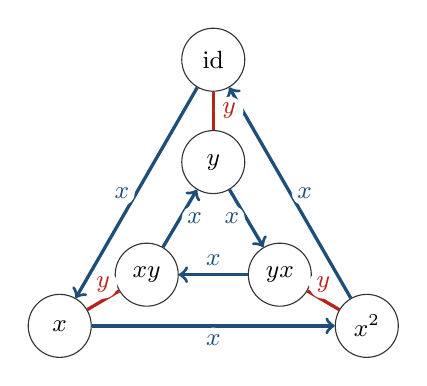
\begin{tikzpicture}[
		scale=0.65,
		every node/.style={circle,draw=darkgray,fill=white,minimum size=8mm,
			inner sep=1pt,font=\small},
		edge label/.style={draw=none,fill=white,minimum size=0pt,inner sep=1pt}
		]
		\node (e)  at (0,3.2)    {$\id$};
		\node (x)  at (-3,-2)    {$x$};
		\node (x2) at (3,-2)     {$x^2$};
		\node (y)  at (0,1.2)    {$y$};
		\node (xy) at (-1.3,-1)  {$xy$};
		\node (yx) at (1.3,-1)   {$yx$};

		\draw[->,very thick,courseblue] (e) -- node[edge label,left] {$x$} (x);
		\draw[->,very thick,courseblue] (x) -- node[edge label,below] {$x$} (x2);
		\draw[->,very thick,courseblue] (x2) -- node[edge label,right] {$x$} (e);
		\draw[->,very thick,courseblue] (y) -- node[edge label,left] {$x$} (yx);
		\draw[->,very thick,courseblue] (yx) -- node[edge label,above] {$x$} (xy);
		\draw[->,very thick,courseblue] (xy) -- node[edge label,right] {$x$} (y);

		\draw[very thick,BrickRed] (e) -- node[edge label,right] {$y$} (y);
		\draw[very thick,BrickRed] (x) -- node[edge label,above] {$y$} (xy);
		\draw[very thick,BrickRed] (x2) -- node[edge label,above] {$y$} (yx);
	\end{tikzpicture}
\end{minipage}


 \section{Recollections on Subgroups}

 \begin{definition}[Subgroup]
	 Let $(G,\cdot,e)$ be a group. A subset $H\subseteq G$ is a \emph{subgroup}
	 if it satisfies the following conditions:
	 \begin{enumerate}[label=\textbf{(\arabic*)}]
		 \item $e\in H$.
		 \item $H$ is closed under products: if $h_1,h_2\in H$, then $h_1h_2\in H$.
		 \item $H$ is closed under inverses: if $h\in H$, then $h^{-1}\in H$,
		 where the inverse is taken in $G$.
		 \end{enumerate}
	 \end{definition}

 A subgroup is itself a group under the same operation, with the same
 identity as $G$. Associativity is inherited from $G$. Recall that we also proved the following result earlier in Lecture 2.

 \begin{proposition}[Finite subgroup criterion]
	 If $H\subseteq G$ is finite, contains $e$, and is closed under products,
	 then $H$ is a subgroup. In this case, closure under inverses follows from
	 the other two conditions.
	 \end{proposition}


 \begin{remark}
	 For an infinite subset, closure under inverses must still be checked.
	 For example, $\{0,1,2,\ldots\}\subseteq(\Z,+,0)$ contains the identity
	 and is closed under addition, but it is not closed under additive inverses.
	 \end{remark}


 Recall that we have also already introduced the following notion.

 \begin{definition}[Cyclic subgroup]
	 Let $G$ be a group, with identity denoted by $1$, and let $x\in G$.
	 The \emph{cyclic subgroup generated by $x$} is
	 \be
	 \langle x\rangle=\{x^m:m\in\Z\}
	  =\{1,x^{\pm1},x^{\pm2},x^{\pm3},\ldots\}.
	 \ee
	 \end{definition}

 We generalize this definition as follows.

 \begin{definition}[Subgroup generated by a subset]
	 For a subset $W\subseteq G$, let $\langle W\rangle$ be the set of all
	 finite products
	 \be
	 w_1w_2\cdots w_k,\qquad k\geq0,
	 \ee
	 where each factor $w_i$ is an element of $W$ or the inverse of an element
	 of $W$. Repetitions are allowed, and the order of the factors matters.
	 When $k=0$, the product is the identity $1$. This is called the
	 \emph{subgroup generated by $W$}.
	 \end{definition}

 Indeed, concatenating two such products gives another such product. As for inverses, let's mention the following important but simple identity that you may remember from a course in linear algebra.
 \be
 (w_1w_2\cdots w_k)^{-1}=w_k^{-1}\cdots w_2^{-1}w_1^{-1}
 \ee
 The product on the right is again of the required form. Hence
 $\langle W\rangle$ is a subgroup.

 \begin{remark}
	 The subgroup $\langle W\rangle$ is the \emph{smallest subgroup containing
		 $W$}. Indeed, it contains $W$ by taking products of length one. If $H$ is
	 any subgroup containing $W$, then closure under inverses and products
	 implies that $H$ contains every product used to define $\langle W\rangle$.
	 Thus $\langle W\rangle\subseteq H$.
	 \end{remark}

 \begin{example}[Subgroups of the integers]
	 In the additive group $(\Z,+,0)$, the even integers, $\{0\}$, and $\Z$
	 are all subgroups. More generally, for $a\in\Z$,
	 \be
	 \Z a=\langle a\rangle=\{ma:m\in\Z\}
	  =\{0,\pm a,\pm2a,\pm3a,\ldots\}
	 \ee
	 is the subgroup consisting of all multiples of $a$.
	 Here the operation is addition, so powers in multiplicative notation
	 become integer multiples in additive notation.
	 \end{example}

 \begin{definition}
	 For any group $G$, the set $\{e\}$ is a subgroup, called the
	 \emph{trivial subgroup}. The whole group $G$ is also a subgroup of itself. A subgroup $H$ is called a \emph{proper subgroup} if $H\neq G$.
	 If $\{e\}\subsetneq H\subsetneq G$, then $H$ is called a \emph{nontrivial proper
		 subgroup}.

	 \end{definition}

 Intersecting subgroups provides another useful way to manufacture new groups.


 \begin{proposition}
	 If $H$ and $K$ are subgroups of $G$, then $H\cap K$ is a subgroup of $G$.
	 \end{proposition}

 \begin{proof}
	 Since $e\in H$ and $e\in K$, we have $e\in H\cap K$.
	 If $a,b\in H\cap K$, then $ab\in H$ and $ab\in K$, because both
	 subgroups are closed under products. Thus $ab\in H\cap K$.
	 Similarly, if $a\in H\cap K$, then $a^{-1}\in H$ and $a^{-1}\in K$,
	 so $a^{-1}\in H\cap K$.
	 \end{proof}

 \begin{remark}
	 The union $H\cup K$ need not be a subgroup. For example,
	 $2\Z\cup3\Z$ contains $2$ and $3$, but does not contain their sum $5$.
	 \end{remark}


\section{Subgroups of \texorpdfstring{$\Z$}{Z} and greatest common divisors}

\begin{lemma}
	Every subgroup of $(\Z,+,0)$ is either $\{0\}$ or $\Z d$ for some
	positive integer $d$.
\end{lemma}

\begin{proof}
	Let $H\subseteq\Z$ be a subgroup with $H\neq\{0\}$. Since $H$ contains
	a nonzero integer and its negative, it contains a positive integer.
	By the well-ordering principle, $H$ has a smallest positive element $d$.
	We claim that $H=\Z d$.

	First, $\Z d\subseteq H$, since $d\in H$ and $H$ is closed under
	addition and additive inverses.

	For the reverse inclusion, let $m\in H$. By division with remainder,
	write
	\be
	m=qd+r,\qquad q\in\Z,\quad 0\leq r<d.
	\ee
	Since $m,qd\in H$, we have $r=m-qd\in H$. If $r>0$, this contradicts
	the choice of $d$ as the smallest positive element of $H$. Thus $r=0$,
	so $m=qd\in\Z d$. Hence $H\subseteq\Z d$, proving the claim.
\end{proof}

\subsection*{Greatest common divisors}

Let $a,b\in\Z$ be not both zero. Consider the set of all integer linear combinations
of $a$ and $b$:
\be
\Z a+\Z b=\{ma+nb:m,n\in\Z\}.
\ee
This is a subgroup of $(\Z,+,0)$: it contains $0$, and sums and negatives
of integer linear combinations are again integer linear combinations.
Therefore the preceding lemma gives
\be
\Z a+\Z b=\Z d
\ee
for some $d>0$, since this subgroup contains a nonzero element.
We will show that this positive generator is $\gcd(a,b)$.

\begin{lemma}[Divisibility and inclusion]\label{lem:divisibility}
	For integers $r,s$,
	\be
	r\mid s\quad\Longleftrightarrow\quad\Z s\subseteq\Z r.
	\ee
\end{lemma}

\begin{proof}
	If $s=kr$ for some $k\in\Z$, then every multiple of $s$ is a multiple
	of $r$. Conversely, if $\Z s\subseteq\Z r$, then $s\in\Z r$, so $r\mid s$.
\end{proof}

\begin{example}
	The direction of inclusion reverses the order in the divisibility relation:
	\be
	2\mid6,\qquad 6\Z\subseteq2\Z.
	\ee
	Indeed, every multiple of $6$ is a multiple of $2$.
\end{example}

\begin{proposition}
	Let $a,b\in\Z$ be not both zero, and let $d>0$ satisfy
	$\Z a+\Z b=\Z d$. Then $d=\gcd(a,b)$. In particular,
	\be
	\Z a+\Z b=\Z\gcd(a,b).
	\ee
\end{proposition}

\begin{proof}
	We check two properties:
	\begin{enumerate}[label=\textbf{(\arabic*)}]
		\item $d$ divides both $a$ and $b$.
		\item Every common divisor of $a$ and $b$ divides $d$.
	\end{enumerate}
	For the first property, the inclusions
	\be
	\Z a\subseteq\Z a+\Z b=\Z d,
	\qquad
	\Z b\subseteq\Z a+\Z b=\Z d
	\ee
	imply $d\mid a$ and $d\mid b$ by Lemma~\ref{lem:divisibility}.

	For the second property, suppose $\ell\mid a$ and $\ell\mid b$.
	Then $\Z a\subseteq\Z\ell$ and $\Z b\subseteq\Z\ell$. Adding elements
	from these two subgroups gives
	\be
	\Z d=\Z a+\Z b\subseteq\Z\ell.
	\ee
	By Lemma~\ref{lem:divisibility}, $\ell\mid d$.
	Every positive common divisor $\ell$ divides $d$, so $\ell\leq d$.
	Since $d$ itself divides both $a$ and $b$, it is their greatest common divisor.
\end{proof}

This gives B\'ezout's identity.

\begin{corollary}[B\'ezout's identity]
	Let $a,b\in\Z$ be not both zero. There exist integers $m,n$ such that
	\be
	\gcd(a,b)=ma+nb.
	\ee
\end{corollary}

\begin{proof}
	Set $d=\gcd(a,b)$. Since $\Z a+\Z b=\Z d$ and $d\in\Z d$, we have
	$d\in\Z a+\Z b$. By the definition of this subgroup, $d=ma+nb$ for some
	$m,n\in\Z$.
\end{proof}



\end{document}
